%%
%% Meta: Boxplot erstellen. Viele Beispiele
%%

\input{bmsLayoutPage}

\renewcommand{\metaHeaderLine}{Arbeitsblatt}
\renewcommand{\arbeitsblattTitel}{Boxplot}

%%%%%%%%%%%%%%%%%%%%%%%%%%%%%%%%%%%%%%%%%%%%%%%%%%%%%%%%%%%%%%%%%%

%\usepackage{amssymb} 
\usepackage{cancel}

\newcommand\Ccancel[2][black]{\renewcommand\CancelColor{\color{#1}}\cancel{#2}}


\begin{document}%%
\arbeitsblattHeader{}
\section{Boxplot}
Erstellen Sie Boxplots...

\TRAINER{Trainer-Version (Lösungen jeweils unten.)}

\begin{itemize}
\item Finden Sie zunächst jeweils den Median und die beiden Quartile
(M, Q1, Q3).
\item Geben Sie die Skala an (dafür ist jeweils eine Linie
vorgesehen).
\item Zeichnen Sie Median und die beiden Quartile ein und schließen
Sie die Box.
\item Berechnen Sie IQR (Interquartilsrange) $\textrm{IQR} = \textrm{Q3} - \textrm{Q1}$
\item Berechnen Sie den 1.5fachen Interquartilsabstand
($1.5\cdot{}(\textrm{Q3}-\textrm{Q1}) = 1.5 \cdot \textrm{IRQ}$).
\item Zeichnen Sie fein (so dass Sie es wieder ausradieren können) die beiden
Ausreißerschwellen ein. Diese liegt beim 1.5fachen Quartilsabstand
unter bzw über der Box.
\item Zeichnen Sie die Whisker\footnote{Erinnert an Whiskas?}
(Antennen, Fühler) und  allfällige Ausreißer als kleine Ringe ein.
\end{itemize}

\newcommand{\boxplot}[2]{
\subsection{Daten}
\begin{tabular}{#1}
\hline
#2\\
\hline
\end{tabular}

\subsubsection*{Boxplot}
\noTRAINER{\mmPapier{1.6}}
}%% end definition "BOXPLOT"


\boxplot{|c|c|c|c|c|c|c|}{7&8&8&9&11&15&21}
\TRAINER{Lösung
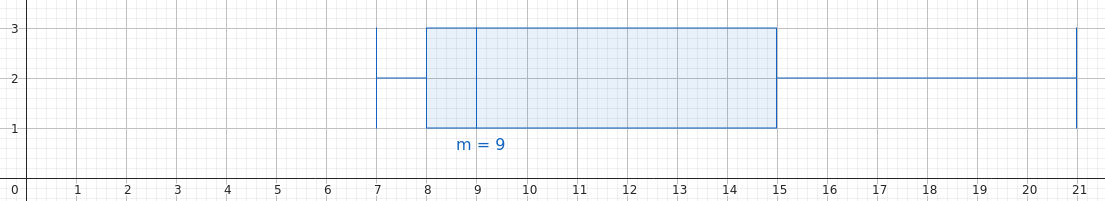
\includegraphics[width=12cm]{img/plot1.png}
}



\boxplot{|c|c|c|c|c|c|c|c|}{7&8&8&9&9&11&15&21}
\TRAINER{Lösung
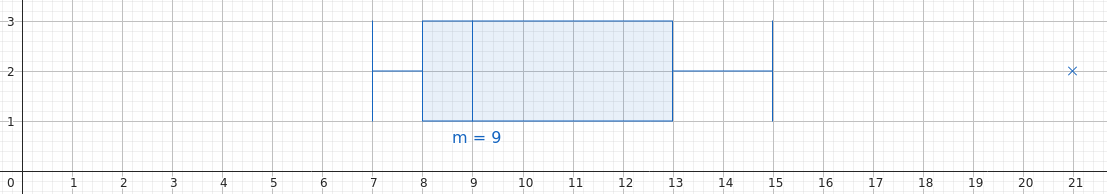
\includegraphics[width=12cm]{img/plot2.png}
}

\newpage
\boxplot{|c|c|c|c|c|c|c|c|c|}{1&7&8&8&9&9&11&15&25}
\TRAINER{Lösung
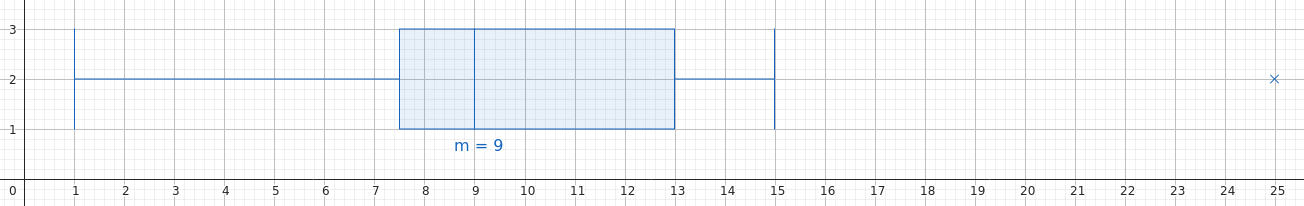
\includegraphics[width=12cm]{img/plot3.png}
}

\boxplot{|c|c|c|c|c|c|c|c|c|c|}{7&8&8&9&9&11&15&21&22&45}
\TRAINER{Lösung
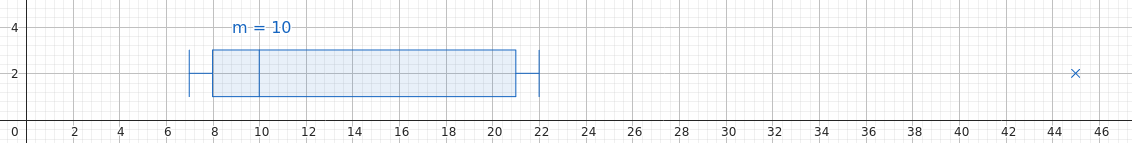
\includegraphics[width=12cm]{img/plot4.png}
}

\boxplot{|c|c|c|c|c|c|c|c|c|c|c|}{23&50&95&96&98&101&102&106&106&112&150}
\TRAINER{Lösung
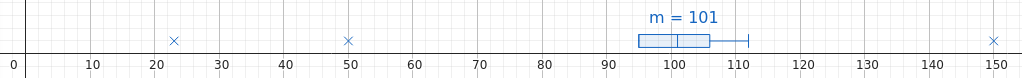
\includegraphics[width=12cm]{img/plot5.png}
}
\newpage


\section{Interpretation}
Interpretieren Sie den folgenden Boxplot.
\begin{center}
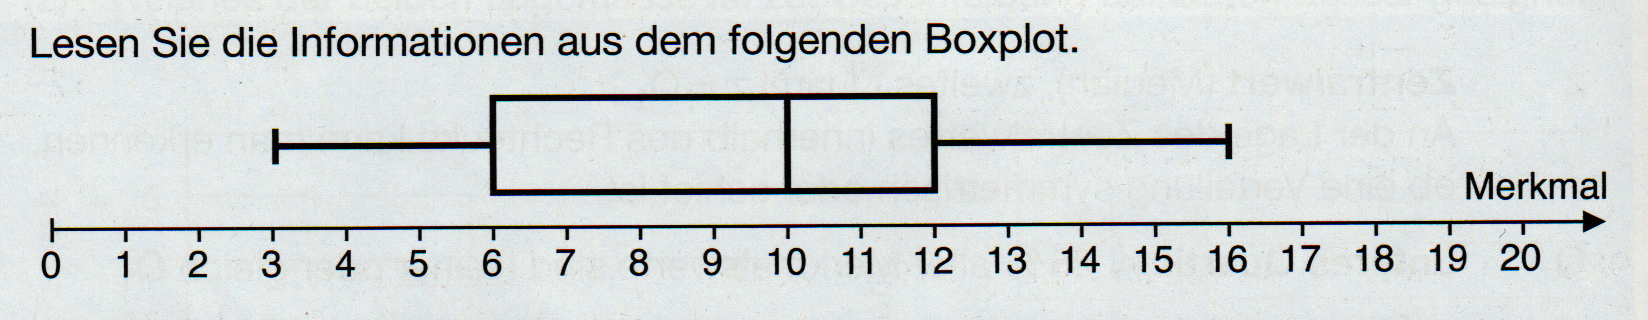
\includegraphics[width=15cm]{img/BoxplotAufgabeFrommenwiler.png}
\end{center}


Q1 = \LoesungsRaum{6}

IQR = \LoesungsRaum{6}

Median = \LoesungsRaum{10}

Obere Ausreißerschwelle = \LoesungsRaum{21}

Spannweite = \LoesungsRaum{13}

Wie viele Prozent der Daten liegen mind zwischen den Werten 3 und
12? \LoesungsRaum{75\%}

\TRAINER{Achtung: Zur Spannweite gehören die Ausreißer dazu!}

\newpage
\subsection{Berechnung}
Von einem Boxplot ist der Median und IQR (Quartilsdifferenz) bekannt:

$$\tilde{x} = 82$$
$$\text{IQR} = 22$$

Sicher kein Ausreißer ist $81$. Doch wie sieht es mit den folgenden
Zahlen aus?

\newcommand{\BoxT}{\TRAINER{\color{green} x}\noTRAINER{\Box}}

(Mit «unterbestimmt» ist gemeint, dass zum Lösen dieser Aufgabe zu
wenig Information vorhanden ist.)

\begin{bbwFillInTabular}{cccc}
Zahl  & sicher Ausreißer & sicher kein Ausreißer & unterbestimmt\\
  4   &   $\BoxT$        & $\Box$                & $\Box$ \\
 26   &   $\BoxT$        & $\Box$                & $\Box$ \\
133   &   $\Box$         & $\Box$                & $\BoxT$ \\
146   &   $\BoxT$        & $\Box$                & $\Box$ \\
 52   &   $\Box$         & $\BoxT$                & $\Box$ \\
114   &   $\Box$         & $\BoxT$                & $\Box$ \\
 44   &   $\Box$         & $\Box$                & $\BoxT$ \\
\end{bbwFillInTabular}

\TRAINER{Die Box liegt minimal bei 60 bis 82 und maximal bei 82 bis
  104. Somit liegen die Ausreißerschwellen minimal bei 27 bis 115 und
  maximal bei 49 bis 137}
\newpage
Von einem Boxplot ist der Median und Q1 (untere 25\%-Quantilsgrenze =
Grenze des ersten Quartils) bekannt:

$$\tilde{x} = 21$$
$$\text{Q1} = 17$$

Sicher kein Ausreißer ist $18$. Doch wie sieht es mit den folgenden
Zahlen aus?

(Mit «unterbestimmt» ist gemeint, dass zum Lösen dieser Aufgabe zu
wenig Information vorhanden ist.)

\begin{bbwFillInTabular}{cccc}
Zahl  & sicher Ausreißer & sicher kein Ausreißer & unterbestimmt\\
 26   &   $\Box$        & $\BoxT$                & $\Box$ \\
 12   &   $\Box$        & $\BoxT$                & $\Box$ \\
 29   &   $\Box$         & $\Box$                & $\BoxT$ \\
1001  &   $\Box$         & $\Box$                & $\BoxT$ \\
\end{bbwFillInTabular}


\end{document}
